\documentclass[a4paper,10pt]{article}
\usepackage{latexsym}
\usepackage[american]{babel}
\usepackage{lmodern}
\usepackage[utf8x]{inputenc}
\usepackage[T1]{fontenc}
\usepackage{longtable}
%\usepackage[dvips]{graphicx}
\usepackage{graphicx}

%\usepackage[pdftex]{hyperref}
\usepackage{hyperref}
\usepackage{amsmath}  % for equation environment
\usepackage{enumitem} % nolistsep to reduce list spacing

\usepackage{parskip} % no indentation in paragraphs

%opening
\title{Automated test generation for {\tt ctsa}}
\author{@hgfernan}
\frenchspacing

\pagestyle{myheadings}

\markboth{Automated test generation for {\tt ctsa}}
         {Automated test generation for {\tt ctsa}}

\addtolength{\hoffset}{-1,5cm}
\addtolength{\textwidth}{+3.5cm}

\addtolength{\voffset}{-1,2cm}
\addtolength{\marginparwidth}{-0,5cm}
\addtolength{\textheight}{+3.5cm}

% \linespread{1.5}


\begin{document}

\maketitle

\begin{abstract}
A routine for the automated test generation for the statistical
library {\tt ctsa} is outlined. It envolves the generation of
simple tasks of model fitting and prediction using {\tt ctsa},
compared with equivalent code in the Python libraries
{\tt pmdarima} and stats models, {\tt simple}, and in the R
library {\tt forecast.}
\end{abstract}

\section{Motivation}

\section{Introduction}

{\em Overview}

\section{Tables}

Since the automated test generation is based on a database, here
follows a description of the database to be used.

It has a mixed relational and document architecture: the main
tables follow a conventional relational structure, but the
parameters and test results are stored as JSON values. That's for
pragmatic reasons: the parameters and test results are varied and
have different structures. That could be easily mapped to a
relational database structure, but it would be too laborious and
cumbersome.

As such, test parameters and results will be stored as JSON
objects encoded as strings, and dealt with by classes specialized
in their content. That is:  an $ARIMA$ model will have three basic
parameters, while a $SARIMA$ model will have 7 basic parameters.
There will be a class for each one of the models, that will be
able to unpack and allow the use those JSON values.

\begin{figure}[h]
    \centering
    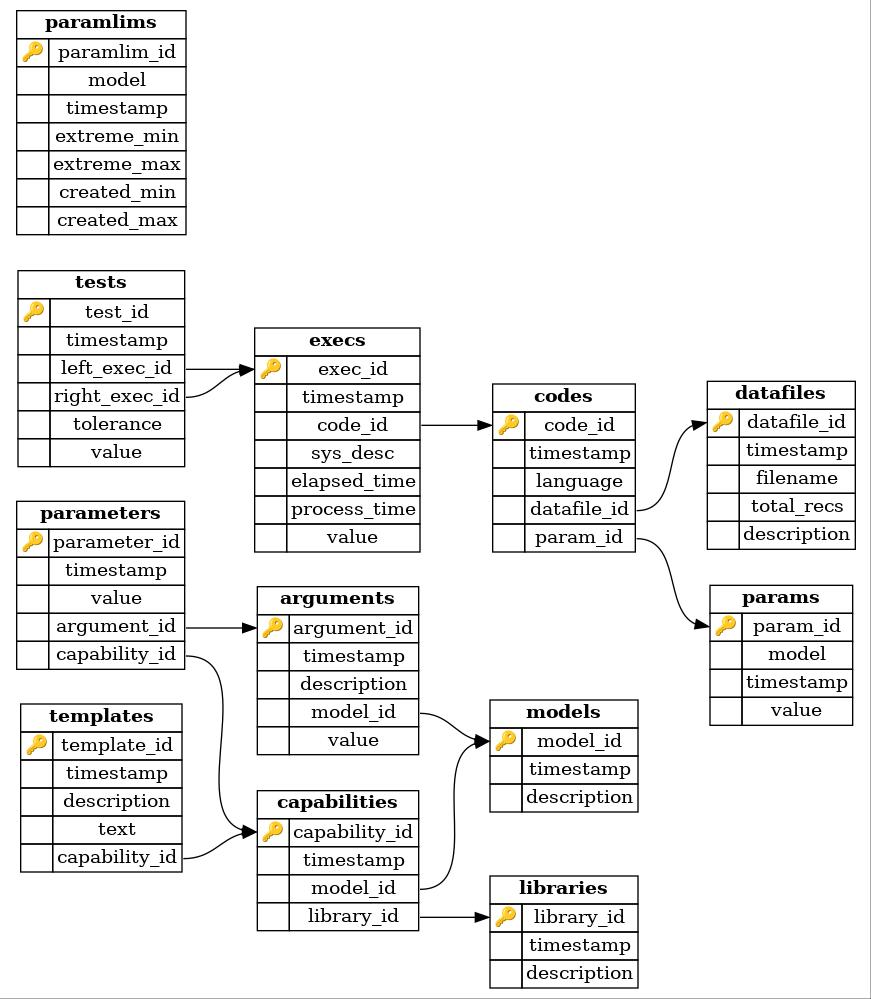
\includegraphics[scale=0.35]
        {../img/schema.jpg}
    \caption{Database used for automated test generation}
    \label{fig:schema}
\end{figure}

In a few words, the algorithm to generate tests follow this way:

\begin{enumerate}
    \item The table {\tt paramlims} (on the upper left corner of
        Figure \ref{fig:schema}) is used to select a sequence of
        parameters for each model, according to the limits present
        in the fields {\tt extreme\_min} and {\tt extreme\_max}.
        They are stored in the table {\tt params} to be detailed
        below.

        Not all parameters are generated, and the range of the
        parameters created are saved in the fields
        {\tt created\_min} and {\tt created\_max}.

        The field {\tt timestamp} contains the last alteration
        of any or all values in the range {\tt created\_min} and
        {\tt created\_max} for its corresponding {\tt model};

    \item The list of data files available (stored in the folder
        {\tt data/}) are listed and each name is contained in the
        field {\tt filename} of the table {\tt datafiles}. In this
        table the date of each file inclusion is recorded in the
        field {\tt timestamp}. The field {\tt total\_recs} of the
        same table contain the number of records of each file.
        The field {\tt description} can be used to introduce
        details of the file: its origin, the transformations used
        to generate it, etc.

    \item There are simple templates for each model, and they're
        used to generate a single file for each of the elements of
        the cartesian product between the allowed range of
        {\tt params} for each model, and the data files in
        {\tt datafiles}.

        This process is replicated for each of the languages in
        use (C, Python, and R) and their corresponding libraries
        {\tt ctsa}, {\tt pmdarima} and {\tt statsmodels}, and
        {\tt forecast}, Those results are storeed in the table
        {\tt codes};

    \item


\end{enumerate}


\end{document}
